% !TeX root = ../thuthesis-example.tex

\chapter{服务器端高性能 \emph{insertRecords} 写入机制设计与实现}
经过客户端的预处理与 RPC 层的数据传输,写入请求最终会到达服务器端。服务器端对写入请求进行预处理后,交由存储引擎负责处理写入请求,并将这些数据最终持久化到磁盘上,服务器端的设计与实现对写入性能有至关重要的影响。如 \ref{sec:chap3-sec3-1} 中的实验结果所示,现有 IoTDB 服务器端对写入请求的处理有较大的性能瓶颈,不能满足高并发写入请求的需求。因此,本章将介绍对 \emph{insertRecords} 写入请求所设计的服务器端高性能写入机制。


\section{服务器端 \emph{insertRecords} 写入流程总览}
\ref{sec:chap3-sec2} 节介绍了 IoTDB 服务器端对 \emph{insertRecords} 写入请求执行的总体流程,新的执行流程和原有流程大体相似,单针对之前实验中发现的瓶颈,本工作进行了重新设计以优化写入性能。

\begin{figure}
  \centering
  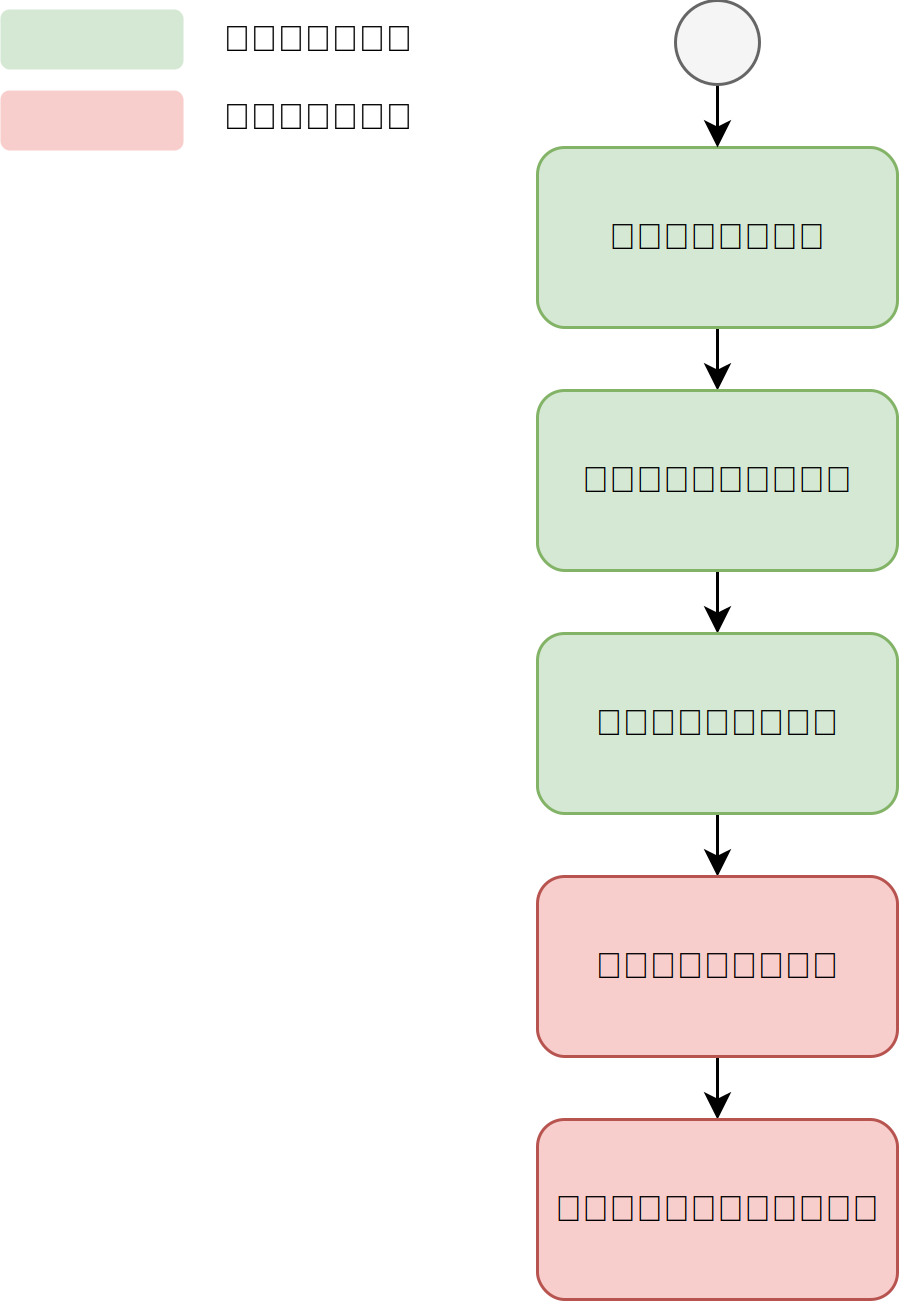
\includegraphics[width=0.9\linewidth]{new-storage-engine.pdf}
  \caption{服务器端 \emph{insertRecords} 写入流程}
  \label{fig:iotdb-insertRecords-flow}
\end{figure}

图 \ref{fig:iotdb-insertRecords-flow} 展示了 \emph{insertRecords} 写入请求到达 IoTDB 服务器端以后的总体执行流程,其中绿色部分代表这些流程与 IoTDB 原有设计基本保持一致,因为它们并不是写入的瓶颈所在;红色部分代表了在原有实现中存在的性能瓶颈,本工作对这些部分进行了重新设计与实现以提高写入性能。


在执行分布式写入计划时,一个写入请求会被分为多个写入计划分片(称为 FragmentInstance,FI),每个分片都是写入到一个 DataRegion 中的计划。根据 DataRegion 的分布,可以将其分为本地 DataRegion 和远程 DataRegion,本地 DataRegion 是指存储引擎所在的节点上的 DataRegion,远程 DataRegion 是指存储引擎所在节点以外的 DataRegion。为了充分利用多核 CPU 的计算能力,本工作将写入本地和写入远程 DataRegion 的过程都设计为了多线程并行执行,以提高写入性能。

在存储引擎写入单个计划分片时,不仅需要将数据记录到内存表中,还需要执行记录写前日志、更新监控信息、维护内存索引等操作。这些操作大部分都不是核心的写入操作,但是却会对写入性能产生较大的影响。因此,本工作通过批量化的形式,将这些操作的代价分摊到多行写入记录上,以减少这些操作对写入性能的影响。例如,原本每写入一行记录就需要记录一次写前日志、更新一次监控信息、维护一次内存索引,现在可以将这些操作批量化,每写入一批记录才执行一次这些操作,这样平均到每一条记录上的代价就大大减小了。最后,为了改善前文提到的使用 \emph{insertRecords} 接口进行写入时写前日志过多的问题,本工作对写前日志进行了压缩,减少了写前日志对磁盘的写入量,提高了写入性能。下面将详细介绍这些优化措施的设计与实现。

\section{多线程并行写入设计与实现}
\subsection{多线程并行写入设计}
图 \ref{fig:fi-parallel-write} 展示了 FragmentInstance 多线程并行写入的总体架构。多线程并行写入的设计分为写入本地 DataRegion 和写入远程 DataRegion 两部分,下面将分别介绍这两部分的设计。

\begin{figure}
  \centering
  \includegraphics[width=\linewidth]{FragmentInstance写入.pdf}
  \caption{多线程并行写入设计}
  \label{fig:fi-parallel-write}
\end{figure}

在一般的系统中,对一项任务的并行执行通常会构建一个线程池负责此工作,以减少线程创建与销毁的开销,在本工作的设计中遵循了这一种范式。因此,想要实现多线程并行写入,我们首先要确定线程池的大小。如果线程池中的线程数过少,那么无法充分利用多核 CPU 的计算能力,从而无法提高写入性能;如果线程池中的线程数过多,那么会增加线程创建与销毁的开销,反而会降低写入性能。根据线程数与 DataRegion 的个数的比例,可以分为多个线程写一个 DataRegion、一个线程写一个 DataRegion 和一个线程写多个 DataRegion 三种情况。在目前 IoTDB 的设计与实现中,每个 DataRegion 都有一个锁,用于保证对 DataRegion 的读写操作是线程安全的。此外,一个 DataRegion 也对应了一个共识组,共识层为了保证数据的一致性,也持有一个锁。在这样的设计下,针对一个 DataRegion 的写入是串行的,即一次只能有一个线程写入一个 DataRegion。

综合以上因素,本工作选择了一个线程写一个本地 DataRegion 的设计,即每个 DataRegion 都有一个专门的线程负责处理这个 DataRegion 的写入任务。为了处理多个写入请求,每个 DataRegion 的线程都会维护一个写入队列,用于存放待写入的数据。不同写入请求对同一个 DataRegion 的写入任务会被放入同一个队列中,该 DataRegion 对应的写入线程会不断从写入队列中取出任务进行处理。为了避免过多任务堆积,任务队列的大小是有限的,超过了队列的大小后,新的写入请求会被拒绝,并向客户端返回写入失败的信息。写入请求向写入队列提交写入任务后,会获得一个 Future 对象,用于知晓写入任务的执行结果。写入任务执行完成后,Future 对象会被设置为完成状态,并且可以通过 Future 对象获取写入任务的执行结果。

对远程 DataRegion 的写入通过网络发送,在系统内缓存了一个全局的客户端池,它们负责将对远程 DataRegion 写入的 FragmentInstance 异步地发送到对应的节点上,并且返回一个 Future 对象,用于后续的处理。

当写入本地 DataRegion 和远程 DataRegion 的 FragmentInstance 都被异步地分发之后,主写入线程会拿到所有这些 FragmentInstance 对应的 Future 对象,并通过这些对象等待它们全部完成,随后将写入结果返回给客户端。

\subsection{多线程并行写入实现}
为了实现上述的设计,本工作通过一个 FragmentExecutionManager 类来管理每个 DataRegion 的写入。